% Familytreemap User Guide
%
% For PDF output: pdflatex familytreemap.tex
% For HTML output: plastex familytreemap.tex
%
% For Graphics:
% Use PNG format to avoid problems with HTML conversion.
% Recommended size: < 13cm x 18cm (width x height).
% Recommended resolution: 300 dpi.
%
% Use fixed width instead of textwidth, so that plastex can
% recognize the graphics size. For example use
% \includegraphics[width=13cm]{img/haplogroups.png}
% instead of
% \includegraphics[width=\textwidth]{img/haplogroups.png}

\documentclass[12pt,a4paper]{article}
\usepackage[utf8]{inputenc}
\usepackage[english]{babel}
\usepackage[colorlinks=true, urlcolor=blue, linkcolor=blue]{hyperref}
\usepackage{graphicx}

\begin{document}
\title{Familytreemap User Guide}
\author{Dirk Struve\\
phylofriend at projectory.de\\
\href{https://github.com/yogischogi/familytreemap/}{https://github.com/yogischogi/familytreemap/}}
\date{\today}
\maketitle
\tableofcontents


\section{Introduction}

\hfill {\sl For the lost ones.}
\vspace{1em}

\noindent
Familytreemap calculates population frequencies
(relative or absolute) from Family Tree DNA projects.

It's main purpose is to create intensity maps of project members.


\section{Command line options}

Familytreemap is a command line program. It is invoked by

\vspace{1em}
\noindent\texttt{familytreemap <options>}

\vspace{1em}
\noindent Options may be given in arbitrary order.

\begin{description}
\item[-help] Prints available program options.
\item[-totalsin] Totals in: Total number of testers from each country.
\item[-in] Input file that contains a table with Family Tree DNA
  project data in CSV format. This is usually the project spreadsheet
  that lists the STR results.
\item[-col] Number of the column that contains the country names.
\item[-skipheader] Ignore the first line of the input file.
\item[-ln] Applies a logarithm to the number of persons to get a nice logarithmic scale.
\item[-out] Output file that contains population frequencies in
  CSV format.
\item[-sumuk] (sum UK) If \texttt{-sumuk=true} the number of
  testers from England, Wales, Scotland and Northern Ireland
  is added to United Kingdom. Default is \texttt{-sumuk=false}
  because this is the way the data is reported by Family Tree DNA.
\item[-statout] Filename for elaborate statistical information.
\end{description}


\section{Installation}

\subsection{Linux Mint}
\begin{enumerate}
\item Make sure that the Go programming language is installed.
	You can install it by typing\\
	\texttt{sudo apt-get install golang}
\item Read the Go
	\href{http://golang.org/doc/install}{Getting Started}
	guide. Make sure to set your \emph{GOPATH} variable and
	include it in your \emph{PATH} so that Go programs can be
	found.
\item Fetch the familytreemap program with\\
	\texttt{go get github.com/yogischogi/familytreemap}
\item Install the program with\\
	 \texttt{go install github.com/yogischogi/familytreemap}
\end{enumerate}

\subsection{Windows, FreeBSD, Mac OS X}
\begin{enumerate}
\item Read the Go
	\href{http://golang.org/doc/install}{Getting Started}
	guide and install the Go programming language. 
	Make sure to set your \emph{GOPATH} variable and
	include it in your \emph{PATH} so that Go programs can be
	found.
\item Fetch the familytreemap program with\\
	\texttt{go get github.com/yogischogi/familytreemap}
\item Install the program with\\
	 \texttt{go install github.com/yogischogi/familytreemap}
\end{enumerate}


\section{Family Tree DNA projects}

\subsection{First usage}

\begin{enumerate}
\item Go to a Family Tree DNA project on the web and open the
  page containing the DNA results in a web browser.
\item Copy the results into a spreadsheet and save it in
  CSV (Comma Separated Values) format. For this example
  name it \emph{projectdata.csv}.

  If you are an administrator you can directly download the
  spreadsheet from your Family Tree DNA GAP account.

\item Open a command line interpreter and go to the
   directory where your files are.
\item Determine the number of the column which contains
  the countries. Often this is 3, familytreemap's default
  value.
\item Issue a command to test if the program works:\\
  \texttt{familytreemap -in=projectdata.csv -out=result.csv -col=3}\\
  If everything works correctly, the file \emph{result.csv}
  contains a list of countries with the number of testers
  from each country.
\end{enumerate}


\subsection{Calculating relative concentrations}

Until now we have only determined how many persons from each
country took a genetic test. This results in a bias because
Family Tree DNA usually has much more customers from highly
populated Western countries than from the rest of the world.

Often we would like the percentage value of how many persons
from a specific country belong to a certain haplogroup. For
this we must divide the number of persons from that haplogroup
by the total number of testers from the country.

Family Tree DNA does not provide the total number of testers
from each country but it does provide the number of 12-marker
testers. This should be a very good approximation because nearly
every male customer has tested for at least 12 markers.

To view the number of 12-marker testers you can sign into
Family Tree DNA and go to \emph{Ancestral Origins}.

To calculate relative frequencies the Familytreemap program
needs a CSV file that contains the total number of testers
from each country. You have to create this file yourself.
The format is very simple. A basic example looks like this:

\begin{verbatim}
Country,Testers
Belarus,1000
Belgium,2000
Brazil,100
\end{verbatim}

If you save your file as \emph{12-marker-testers.csv}
you can start to calculate a relative distribution by using
the \texttt{-totalsin} option:

\vspace{1ex}
\noindent
\texttt{familytreemap -totalsin=12-marker-testers.csv -in=projectdata.csv -out=result.csv -col=3}
\vspace{1ex}

\noindent
The file \emph{results.csv} should now contain the percentage
value of persons belonging to a specific project or haplogroup
relative to the total number of 12-marker testers from each country.


\subsection{Does England belong to the United Kingdom?}

Family Tree DNA reports the number of testers according to
self reported origins. They do not apply any post-processing.
As a result persons from England, Wales, Scotland and Northern
Ireland are not counted as belonging to the United Kingdom.

To get the correct count Familytreemap provides the 
\texttt{-sumuk} (sum UK) option, which adds the testers from
England, Wales, Scotland and Northern Ireland to the United
Kingdom. Example:

\vspace{1ex}
\noindent
\texttt{familytreemap -totalsin=12-marker-testers.csv -in=projectdata.csv -out=result.csv -col=3 -sumuk=true}


\subsection{Creating a heat map}

\begin{figure}[ht]
\centering
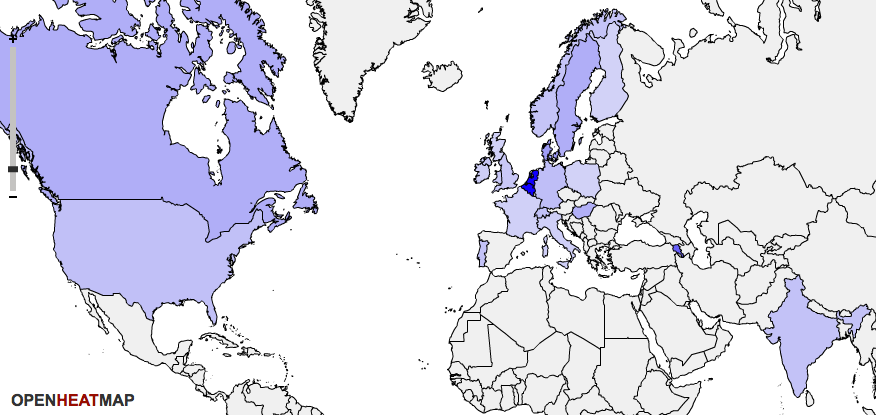
\includegraphics[width=13cm]{heatmap-haplo.png}
\caption{Geographical distribution of persons belonging
to a haplogroup. Created with \href{http://www.openheatmap.com/}{OpenHeatMap}.}
\end{figure}

\begin{enumerate}
\item Run the familytreemap program:\\
  \texttt{familytreemap -totalsin=12-marker-testers.csv -in=projectdata.csv -out=result.csv -col=3 -sumuk=true}
\item Open your web browser and go to
      \href{http://www.openheatmap.com/}{http://www.openheatmap.com}.
	\begin{enumerate}
	\item Click on \emph{Create your map}.
	\item \emph{Excel or CSV file}.
	\item \emph{Upload} your results file,
            in this example \emph{result.csv}.
	\item \emph{View your map} and adjust the settings until you like it.
	\item \emph{Save \& view}
	\end{enumerate}
\item You are done! You can share your map via social networks
  or take a screenshot of it.
\end{enumerate}


\section{MyHeritage matches}

\begin{figure}[ht]
\centering
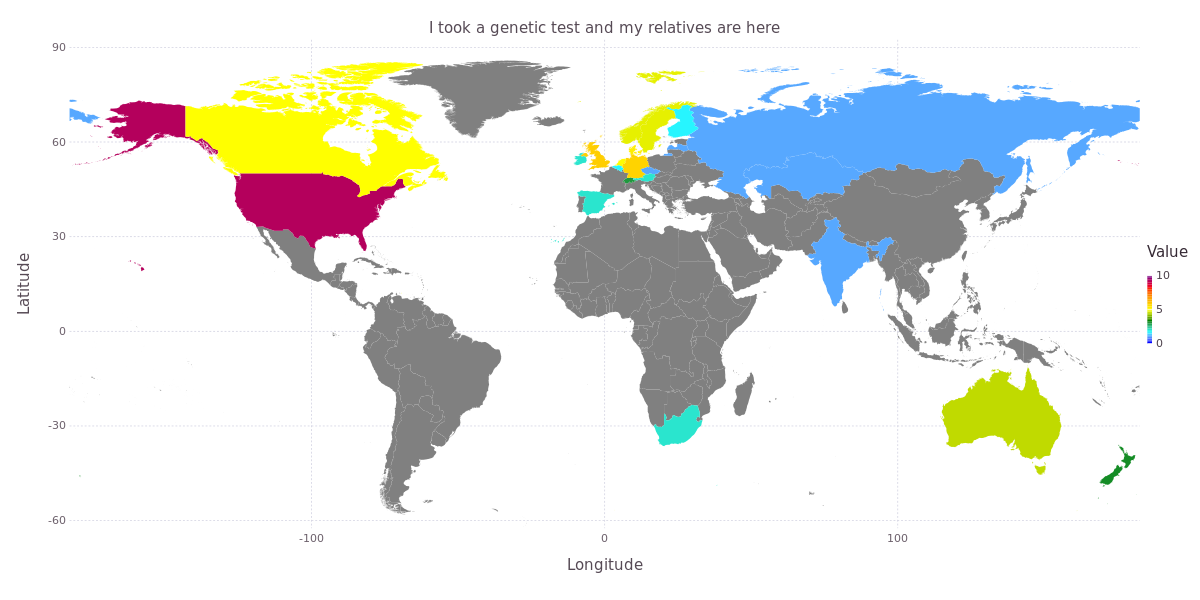
\includegraphics[width=13cm]{heatmap.png}
\caption{Worldwide heatmap of genetic matches.
Created with \href{https://julialang.org/}{Julia},
\href{http://gadflyjl.org/}{Gadfly} and
\href{http://www.naturalearthdata.com/}{Natural Earth}.}
\end{figure}

Familytreemap can also be used to create a heatmap of
MyHeritage matches. One of the easiest options is to use
OpenHeatMap.

\begin{enumerate}
\item Get a list of your matches from MyHeritage
	(MyHeritage $\rightarrow$ DNA $\rightarrow$ DNA Matches
	$\rightarrow$ Advanced options $\rightarrow$ Export DNA Matches list).
\item Run the familytreemap program on your matches list:\\
  \texttt{familytreemap -in=MyHeritage-matches.csv -out=result.csv \\
	-col=4 -skipheader=true}
\item Open your web browser and go to
      \href{http://www.openheatmap.com/}{http://www.openheatmap.com}.
	\begin{enumerate}
	\item Click on \emph{Create your map}.
	\item \emph{Excel or CSV file}.
	\item \emph{Upload} your results file,
            in this example \emph{result.csv}.
	\item \emph{View your map} and adjust the settings until you like it.
	\item \emph{Save \& view}
	\end{enumerate}
\item You are done! You can share your map via social networks
  or take a screenshot of it.
\end{enumerate}








\end{document}
